%  LaTeX support: latex@mdpi.com 
%  In case you need support, please attach all files that are necessary for compiling as well as the log file, and specify the details of your LaTeX setup (which operating system and LaTeX version / tools you are using).

%=================================================================
\documentclass[journal,article,applsci,submit,moreauthors,pdftex]{Definitions/mdpi} 
\graphicspath{ {./images/} }
% If you would like to post an early version of this manuscript as a preprint, you may use preprint as the journal and change 'submit' to 'accept'. The document class line would be, e.g., \documentclass[preprints,article,accept,moreauthors,pdftex]{mdpi}. This is especially recommended for submission to arXiv, where line numbers should be removed before posting. For preprints.org, the editorial staff will make this change immediately prior to posting.

%--------------------
% Class Options:
%--------------------
%----------
% journal
%----------
% Choose between the following MDPI journals:
% acoustics, actuators, addictions, admsci, aerospace, agriculture, agriengineering, agronomy, algorithms, animals, antibiotics, antibodies, antioxidants, applsci, arts, asc, asi, atmosphere, atoms, axioms, batteries, bdcc, behavsci , beverages, bioengineering, biology, biomedicines, biomimetics, biomolecules, biosensors, brainsci , buildings, cancers, carbon , catalysts, cells, ceramics, challenges, chemengineering, chemistry, chemosensors, children, cleantechnol, climate, clockssleep, cmd, coatings, colloids, computation, computers, condensedmatter, cosmetics, cryptography, crystals, dairy, data, dentistry, designs , diagnostics, diseases, diversity, drones, econometrics, economies, education, ejihpe, electrochem, electronics, energies, entropy, environments, epigenomes, est, fermentation, fibers, fire, fishes, fluids, foods, forecasting, forests, fractalfract, futureinternet, futurephys, galaxies, games, gastrointestdisord, gels, genealogy, genes, geohazards, geosciences, geriatrics, hazardousmatters, healthcare, heritage, highthroughput, horticulturae, humanities, hydrology, ijerph, ijfs, ijgi, ijms, ijns, ijtpp, informatics, information, infrastructures, inorganics, insects, instruments, inventions, iot, j, jcdd, jcm, jcp, jcs, jdb, jfb, jfmk, jimaging, jintelligence, jlpea, jmmp, jmse, jnt, jof, joitmc, jpm, jrfm, jsan, land, languages, laws, life, literature, logistics, lubricants, machines, magnetochemistry, make, marinedrugs, materials, mathematics, mca, medicina, medicines, medsci, membranes, metabolites, metals, microarrays, micromachines, microorganisms, minerals, modelling, molbank, molecules, mps, mti, nanomaterials, ncrna, neuroglia, nitrogen, notspecified, nutrients, ohbm, optics, particles, pathogens, pharmaceuticals, pharmaceutics, pharmacy, philosophies, photonics, physics, plants, plasma, polymers, polysaccharides, preprints , proceedings, processes, proteomes, psych, publications, quantumrep, quaternary, qubs, reactions, recycling, religions, remotesensing, reports, resources, risks, robotics, safety, sci, scipharm, sensors, separations, sexes, signals, sinusitis, smartcities, sna, societies, socsci, soilsystems, sports, standards, stats, surfaces, surgeries, sustainability, symmetry, systems, technologies, test, toxics, toxins, tropicalmed, universe, urbansci, vaccines, vehicles, vetsci, vibration, viruses, vision, water, wem, wevj

%---------
% article
%---------
% The default type of manuscript is "article", but can be replaced by: 
% abstract, addendum, article, benchmark, book, bookreview, briefreport, casereport, changes, comment, commentary, communication, conceptpaper, conferenceproceedings, correction, conferencereport, expressionofconcern, extendedabstract, meetingreport, creative, datadescriptor, discussion, editorial, essay, erratum, hypothesis, interestingimages, letter, meetingreport, newbookreceived, obituary, opinion, projectreport, reply, retraction, review, perspective, protocol, shortnote, supfile, technicalnote, viewpoint
% supfile = supplementary materials

%----------
% submit
%----------
% The class option "submit" will be changed to "accept" by the Editorial Office when the paper is accepted. This will only make changes to the frontpage (e.g., the logo of the journal will get visible), the headings, and the copyright information. Also, line numbering will be removed. Journal info and pagination for accepted papers will also be assigned by the Editorial Office.

%------------------
% moreauthors
%------------------
% If there is only one author the class option oneauthor should be used. Otherwise use the class option moreauthors.

%---------
% pdftex
%---------
% The option pdftex is for use with pdfLaTeX. If eps figures are used, remove the option pdftex and use LaTeX and dvi2pdf.

%=================================================================
\firstpage{1} 
\makeatletter 
\setcounter{page}{\@firstpage} 
\makeatother
\pubvolume{xx}
\issuenum{1}
\articlenumber{5}
\pubyear{2019}
\copyrightyear{2019}
%\externaleditor{Academic Editor: name}
\history{Received: date; Accepted: date; Published: date}
%\updates{yes} % If there is an update available, un-comment this line

%% MDPI internal command: uncomment if new journal that already uses continuous page numbers 
%\continuouspages{yes}

%------------------------------------------------------------------
% The following line should be uncommented if the LaTeX file is uploaded to arXiv.org
%\pdfoutput=1

%=================================================================
% Add packages and commands here. The following packages are loaded in our class file: fontenc, calc, indentfirst, fancyhdr, graphicx, lastpage, ifthen, lineno, float, amsmath, setspace, enumitem, mathpazo, booktabs, titlesec, etoolbox, amsthm, hyphenat, natbib, hyperref, footmisc, geometry, caption, url, mdframed, tabto, soul, multirow, microtype, tikz
\usepackage{listings}

%=================================================================
%% Please use the following mathematics environments: Theorem, Lemma, Corollary, Proposition, Characterization, Property, Problem, Example, ExamplesandDefinitions, Hypothesis, Remark, Definition, Notation, Assumption
%% For proofs, please use the proof environment (the amsthm package is loaded by the MDPI class).

%=================================================================
% Full title of the paper (Capitalized)
\Title{An Autonomous and Decentralized Data Marketplace for Trusted Machine Economy $^{\dagger}$}

% Author Orchid ID: enter ID or remove command
\newcommand{\orcidauthorA}{0000-0000-000-000X} % Add \orcidA{} behind the author's name
%\newcommand{\orcidauthorB}{0000-0000-000-000X} % Add \orcidB{} behind the author's name

% Authors, for the paper (add full first names)
\Author{Zan-Jun Wang $^{1}$, Ching-Hua (Vivian) Lin $^{2}$, Yang-Hao Yuan $^{3}$, Zih-shiuan (Spin) Yuan$^{3}$ and Ching-Chun (Jim) Huang$^{2,}$*}

% Authors, for metadata in PDF
\AuthorNames{Zan-Jun Wang, Ching-Hua (Vivian) Lin, Yang-Hao Yuan and Ching-Chun (Jim) Huang}

% Affiliations / Addresses (Add [1] after \address if there is only one affiliation.)
\address{%
$^{1}$ \quad Department of Computer Science and Information Engineering, National Taiwan University\\
$^{2}$ \quad Department of Computer Science and Information Engineering, National Cheng Kung University\\
$^{3}$ \quad BiiLabs Co., Ltd.}

% Contact information of the corresponding author
\corres{Correspondence: jserv@ccns.ncku.edu.tw}

% Current address and/or shared authorship
%\firstnote{Current address: Affiliation 3} 
%\secondnote{These authors contributed equally to this work.}
% The commands \thirdnote{} till \eighthnote{} are available for further notes

%\simplesumm{} % Simple summary

\conference{2019 IEEE Eurasia Conference on IOT, Communication and Engineering (IEEE ECICE 2019), National Formosa University, Yunlin, Taiwan, 3–6 October, 2019} % An extended version of a conference paper

% Abstract (Do not insert blank lines, i.e. \\) 
%%%% 200 words
\abstract{Transacting IoT data must be different in many from traditional approaches in order to build much-needed trust in data marketplaces—trust that will be key to their sustainability. Data generated internally to an organization is usually not enough to remain competitive, enhance customer experiences, or improve strategic decision-making. In this paper, we propose a novel approach to construct IoT-enabled data marketplaces via a decentralized and trustless architecture through the posting of trade records while including the transaction process on distributed ledgers. This approach can efficiently enhance the degree of transparency, as all interactions with smart contracts will be written on-chain. Storage via an end-to-end encrypted message channel allows transmitting and accessing trusted data streams over distributed ledgers regardless of the size or cost of the device, while simultaneously making a verifiable Auth-compliant request to the platform. Furthermore, the platform will complete matching, trading and refunding processes without human intervention which also protects the rights of data providers and consumers through a trading policy written on the smart contract, and finally apply evolutionary game theory to the machine economy.}

% Keywords
\keyword{streaming data; crowd sensing; data marketplace; decentralization}

% The fields PACS, MSC, and JEL may be left empty or commented out if not applicable
%\PACS{J0101}
%\MSC{}
%\JEL{}

%%%%%%%%%%%%%%%%%%%%%%%%%%%%%%%%%%%%%%%%%%
% Only for the journal Diversity
%\LSID{\url{http://}}

%%%%%%%%%%%%%%%%%%%%%%%%%%%%%%%%%%%%%%%%%%
% Only for the journal Applied Sciences:
%\featuredapplication{Authors are encouraged to provide a concise description of the specific application or a potential application of the work. This section is not mandatory.}
%%%%%%%%%%%%%%%%%%%%%%%%%%%%%%%%%%%%%%%%%%

%%%%%%%%%%%%%%%%%%%%%%%%%%%%%%%%%%%%%%%%%%
% Only for the journal Data:
%\dataset{DOI number or link to the deposited data set in cases where the data set is published or set to be published separately. If the data set is submitted and will be published as a supplement to this paper in the journal Data, this field will be filled by the editors of the journal. In this case, please make sure to submit the data set as a supplement when entering your manuscript into our manuscript editorial system.}

%\datasetlicense{license under which the data set is made available (CC0, CC-BY, CC-BY-SA, CC-BY-NC, etc.)}

%%%%%%%%%%%%%%%%%%%%%%%%%%%%%%%%%%%%%%%%%%
% Only for the journal Toxins
%\keycontribution{The breakthroughs or highlights of the manuscript. Authors can write one or two sentences to describe the most important part of the paper.}

%\setcounter{secnumdepth}{4}
%%%%%%%%%%%%%%%%%%%%%%%%%%%%%%%%%%%%%%%%%%
\begin{document}
%%%%%%%%%%%%%%%%%%%%%%%%%%%%%%%%%%%%%%%%%%

%%%%%%%%%%%%%%%%%%%%%%%%%%%%%%%%%%%%%%%%%%

%The order of the section titles is: Introduction, Materials and Methods, Results, Discussion, Conclusions for these journals: aerospace,algorithms,antibodies,antioxidants,atmosphere,axioms,biomedicines,carbon,crystals,designs,diagnostics,environments,fermentation,fluids,forests,fractalfract,informatics,information,inventions,jfmk,jrfm,lubricants,neonatalscreening,neuroglia,particles,pharmaceutics,polymers,processes,technologies,viruses,vision

\section{Introduction}
The growth of data marketplaces is an inevitable result of the IoT (Internet of Things) revolution. As physical assets such as ships, factories, vehicles, farms and buildings become digital, their digital twins will gradually act as secure data exchanges.\cite{digitaltwin}\cite{AutonomousDriving} As data streams surge across silos and carry value across organizations, traditional value chains will transition into a web of value. This paradigm shift will be more complex to administers, forcing businesses to rethink their competitive play as part of these ecosystems. Data marketplaces will emerge as a means to exchange data, monetize data streams and provide the basis of new business models. We refer to this new wave of value creation, for the Internet of Everything, as the "Economy of Things." There are three main barriers to achieving data marketplace:
\begin{enumerate}[leftmargin=*,labelsep=4.9mm]
    \item Data owners do not have much control over their data and their data is locked in silos managed by products and services companies.
    \item Data owners only have access to their own data which has little value when it comes to knowledge discovery.
    \item Data owners do not know how to discover knowledge from raw data.
\end{enumerate}

To overcome these barriers, we implemented IoT-enabled data marketplace and sensor data submission functionalities which are intended to be very lightweight and capable of running on embedded devices. They will only need to perform Tangle operations (e.g., producing and consuming secure channels) and communicate with decentralized facilities, which do not rely on single-source network infrastructure. This proposed reference architecture includes functions that could be mapped to different stakeholders, and multiple functions can be implemented by the same administrative stakeholder in a given operational deployment.
\begin{enumerate}[leftmargin=*,labelsep=4.9mm]
    \item Data Sellers are entities that deploy an IoT infrastructure, for example smart energy meters. These entities are interested in selling the collected data or subsets of that data.
    \item Managed Data Lakes would typically store a massive amount of data and metadata to enable data discovery.
    \item Data Buyers consuming data streams or downloading data sets are interested in the additional value that external data can bring to their internal data.
\end{enumerate}

Looking at Airbox\cite{LASS} as an example, every household with an Airbox device can collect air quality records automatically and autonomically—rather than passively receive the outcomes from the centralized authorities. To protect privacy, data should be encrypted before going on-chain. As for data reliability, we extended the backbone design of the Airbox to interoperate smart-contract-oriented structure to record every transaction. At the same time, data on-chain will send a verifiable request to mark itself as "being tradeable." This step enables buyers to review and bargain at will. Last but not least, payments will be stored on the smart contracts until the transactions are confirmed. The entire sequence is illustrated in Figure \ref{fig:airbox}.

\begin{figure}[h]
    \centering
    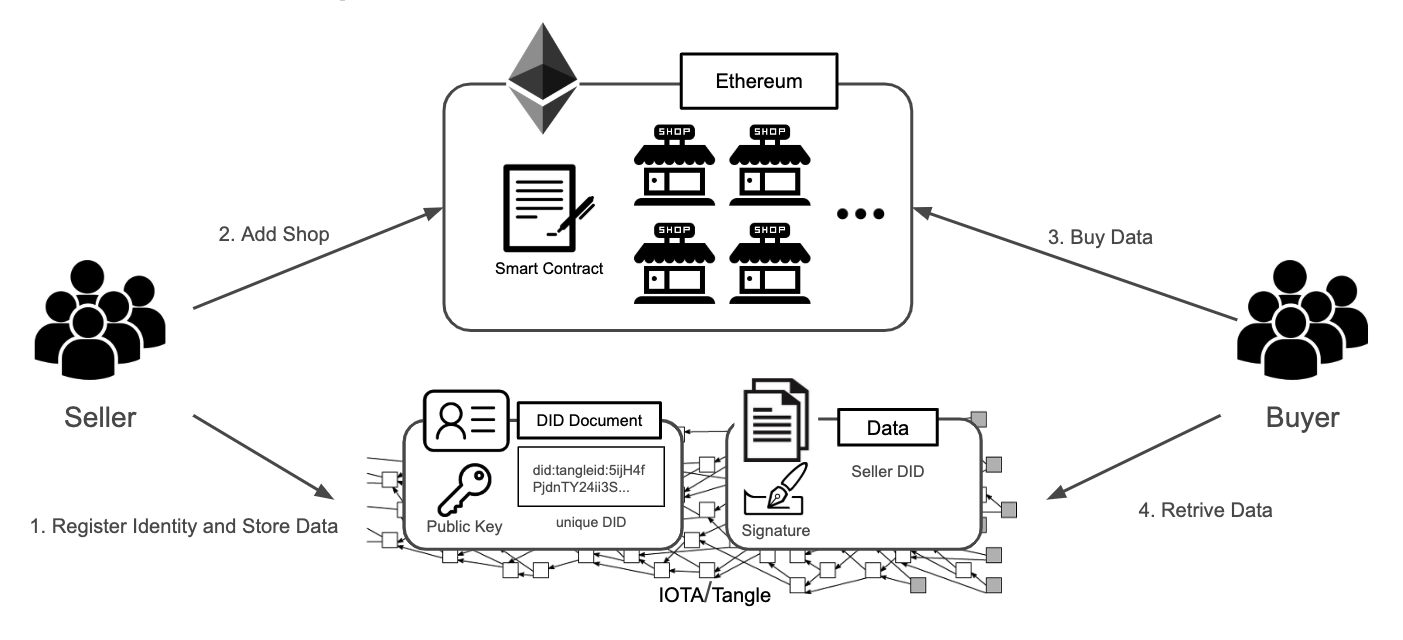
\includegraphics[width=5.5 in]{airbox}
    \caption{IoT-enabled personal air quality assistant.}
    \label{fig:airbox}
\end{figure}
 
%%%%%%%%%%%%%%%%%%%%%%%%%%%%%%%%%%%%%%%%%%
\section{Materials and Methods}
\subsection{Related Work}
As the economic value of huge amounts of data emerges, several researchers have started to explore the design of the data marketplace. The Third Party Auditors (TPAs)-based frameworks\cite{TPA} is far from being satisfactory due to the unstandardized data format and dynamic nature of IoT data. Therefore, a decentralized data integrity validation and trading process has been proposed in recent years, and distributed ledger technology (DLT) is considered a solution, which has the immutable data storage feature that the existence of data can be trusted and no longer rely on any third party authority.

Data Integrity as a Service (DIaaS) is a blockchain based framework for data integrity proposed by Liu et al.\cite{DIaas} which is a Cloud Server Service (CSS) that allows both data provider and consumer to validate data integrity by comparing hashes on Ethereum smart contracts\cite{smartContract} and cloud servers. Moreover, Ethereum smart contract can also realize the purchase agreement, including authorization and penalization. However, the architecture of DIaaS needs high trust on the CSS. If the CSS is malicious or has crashed, losses to both providers and consumers will result. Also, performance analysis shows that IoT devices have low efficiency interactions with Ethereum due to the time-consuming Proof-of-Work (PoW) process.

To address the inefficiency of the Blockchain, \textbf{IOTA}\cite{IOTAwhitepaper} is a cryptocurrency for the IoT industry based on a revolutionary distributed ledger technology, the \textbf{Tangle}, which creates the potential for feeless transactions between users and statistically indefinite network scalability. On top of that, \textbf{Masked Authenticated Messaging(MAM)}\cite{MAM}\cite{MAMSpec}\cite{MAMDescription}, is provided for a second layer data communication protocol which allows transmission, access, and verification of an encrypted data stream over the Tangle where privacy and integrity meet.

Based on Tangle and MAM, the IOTA Foundation launched autonomous and decentralized Industry Marketplace\cite{IOTAIdustryMarketplace} which is suitable for IoT streaming data that not only allows data providers to put data on Tangle without any trusted cloud services, but also allow providers and consumers to trade on Tangle with privacy protection and assurance of data integrity from the source with MAM. Nevertheless, the platform design is centralized, where new devices require manual approval to be visible in the marketplace. Also, interacting with Tangle is still the bottleneck for low-level devices especially in an unstable network or electrically noisy environment.

A different framework design proposed by Gupta, S.Kanhere and Jurdak\cite{3tierDataMarket} could reduce the burden of low-level devices as mentioned. The infrastructure is a 3-tier decentralized data marketplace architectural design with Ethereum smart contracts which consist of providers, consumers and brokers. The broker is a trustless and highly resourced device that will facilitate the trading of data between the consumer and providers. However, the data integrity and authentication of each participant is still forthcoming.

The sustainability of IoT economic system was discussed by Dusit Niyato et al.\cite{UtilityStruct}. They evaluated the utility structure of data trading and presented a game theory model.  Data marketplace organizers can determine their policies to ensure a sustainable system with the Nash Equilibrium found via game theory and its utility structure. However, refund and subscription economies were not mentioned in their work.

Such work proposed different solutions to specific issues of data marketplaces. In this paper, we propose an overall design of decentralized data marketplace that handles data integrity and trading procedures such as buyout and subscriptions to future data on a distributed ledger.

\subsection{System Architecture}
Our proposed data marketplace framework is a 3-tier decentralized architecture with a registrar who is responsible for marketplace registration in order to post participants' information on distributed ledgers for validation, data providers who publish data, data consumers who search for interested products and issue a new trade, and brokers who interact between data providers and consumers, including data publishing, product metadata generation and trading process.

\subsubsection{Participants}
There are four major roles in the decentralized data marketplace (Figure \ref{fig:system_design}).

\begin{itemize}[leftmargin=*,labelsep=5.8mm]
\item \textbf{Registrar: }
The registrar is responsible for creating a Registration Contract, which maintains a lookup table of participants, and has the authority to control the participant lists of the decentralized data marketplace.
\item \textbf{Data Provider: }
Data providers, who generate and preserve streaming data, are willing to sell streaming data to consumers and receive subscription fees from consumers, which can be used to improve the quantity and accuracy of their device or service.
\item \textbf{Consumer: }
Consumers aspire to obtain streaming data to promote the value of their service. However, it is a significant challenge for most consumers to collect the desired data by themselves, so they look to purchasing the streaming data from data providers.
\item \textbf{Broker: }
Brokers represent data providers and consumers to perform computing tasks as brokers are expected to have higher resource. Some trustworthy brokers who pass procedures for conformity assessment are added to the decentralized data marketplace. Once a qualified data provider requests to launch a new product, the broker is requested to deal with the trading process and publish the provider’s data streams to the MAM channel. Brokerage fees for each product will be charged by the broker.
\end{itemize}

\begin{figure}[h]
    \centering
    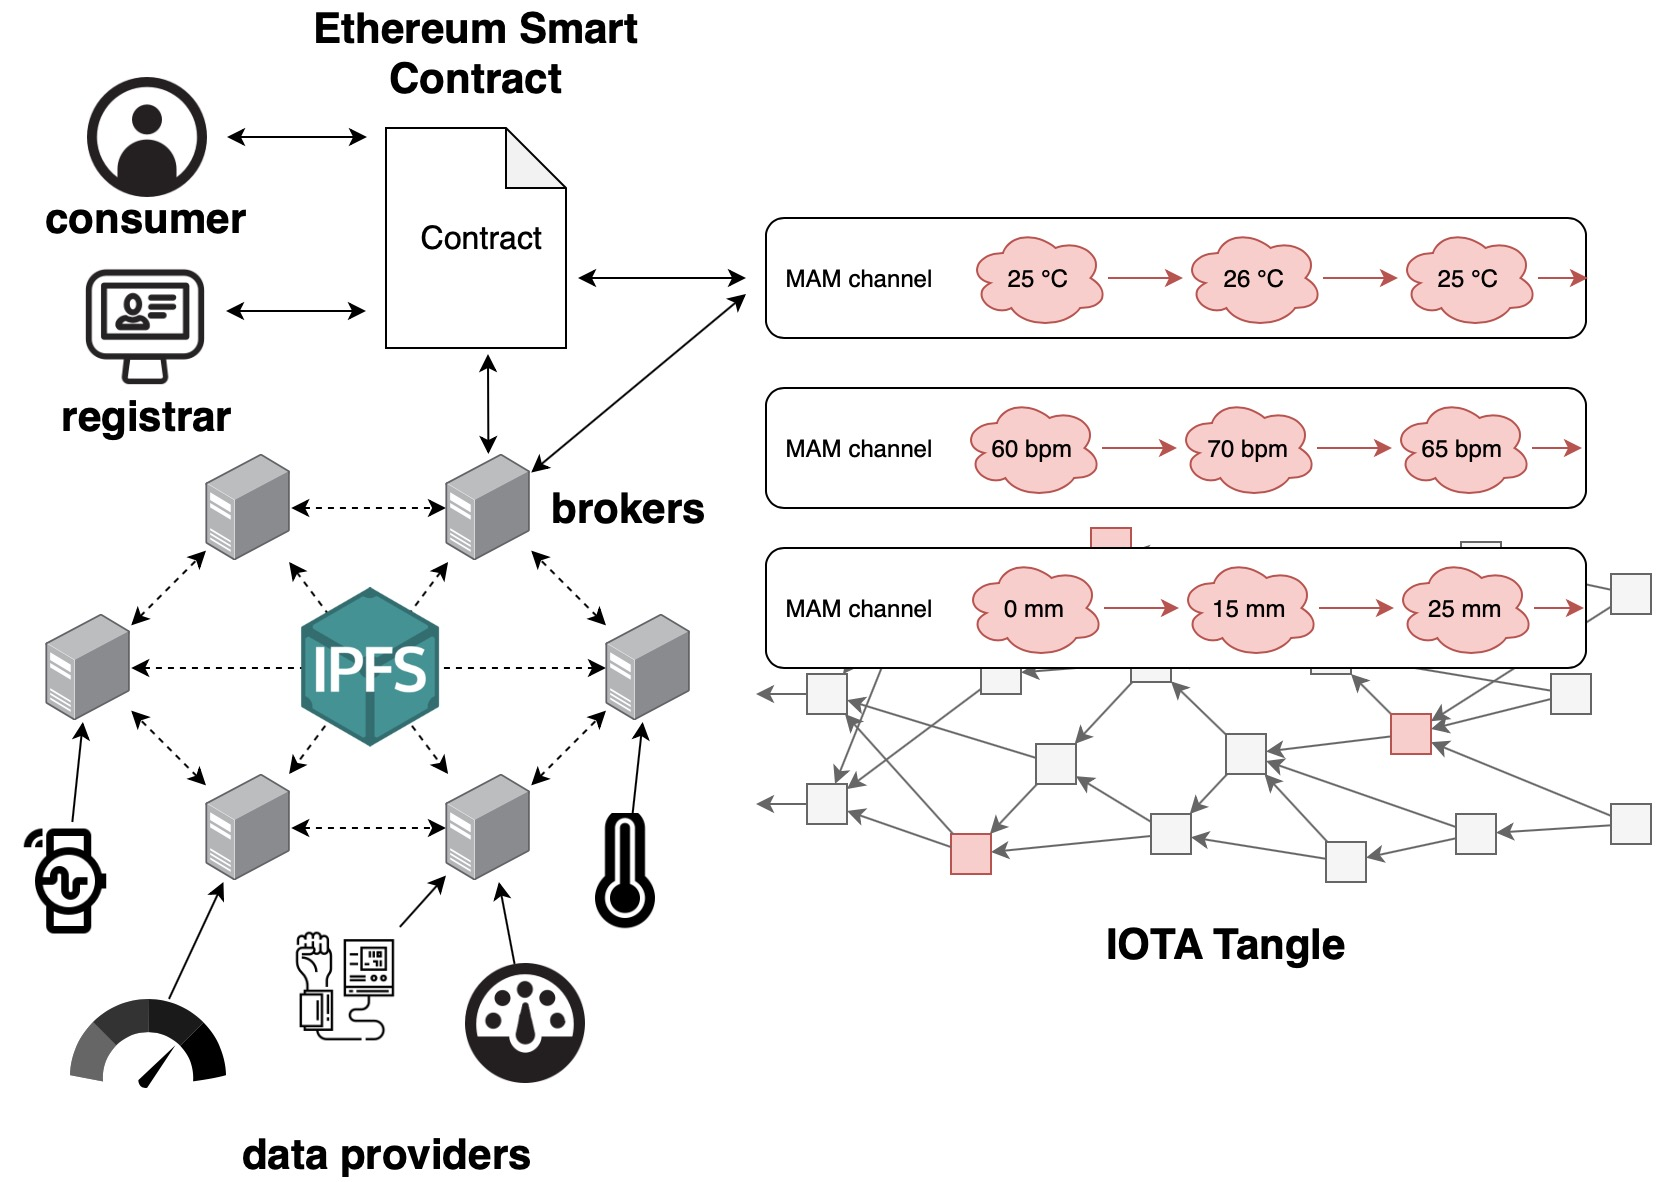
\includegraphics[width=3.3 in]{system_design}
    \caption{The system design of a decentralized architecture which consists of a registrar, data providers, consumers and brokers.}
    \label{fig:system_design}
\end{figure}

\subsubsection{Components}
\begin{itemize}[leftmargin=*,labelsep=5.8mm]
\item \textbf{Mask Authenticated Messaging: }
IOTA is a feeless cryptocurrency designed for IoT while MAM is the second layer data communication protocol built on top of the IOTA network, the Tangle. MAM resolves the challenge of publishing authenticated streaming data as zero-value transactions to distributed ledgers, and provides the ability to publish and fetch encrypted messages over the Tangle along with data integrity and access control.

In IOTA protocol, seed is the identifier of its owner. An IOTA seed represents the ownership of all things associated with the user in the IOTA ecosystem, such as IOTA tokens or messages on the Tangle. With the seed, the owner can produce addresses and signatures in order to issue transactions or publish messages to MAM channels and endpoints.

Either channel or endpoint is like singly-linked list. The MAM channel's ID and endpoint's ID are the addresses of transaction and are the root of a channel and endpoint. Each address of a message can be derived from the previous one. A user can create multiple channels and multiple endpoints under the same channel. The messages can be encrypted with the session key and broadcasted in chronological order to the Tangle by attaching it to an endpoint. This allows only entities that know the session key can decode these messages after retrieving it from the Tangle, and also implements the concept of forward secrecy, where one have no access to the data back from his/hers entry point. Figure \ref{fig:mam_struct} shows the architecture of MAM.

\begin{figure}[H]
    \centering
    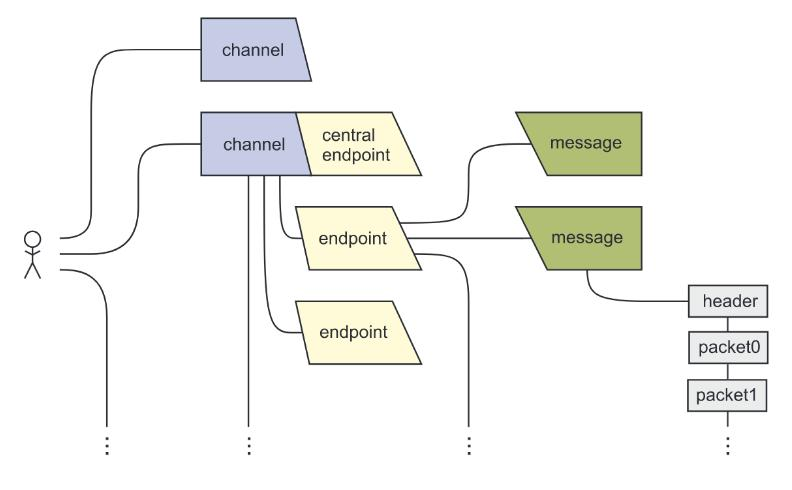
\includegraphics[width=4.4 in]{mam_struct}
    \caption{The concept of MAM.}
    \label{fig:mam_struct}
\end{figure}

The authentication in MAM includes source and data authentication. Source authentication ensures that the message originates from the claimed owner, and data authentication ensures the integrity of the data from that sender. These are achieved through Merkle signature scheme\cite{MSS} (MSS) which is a digital signature scheme based on Merkle Hash Trees and One-way hash functions. However, the size of Merkle Hash Trees should be fixed at start, which is the size of a channel and endpoint is decided before creation. Thus data providers need to firstly decide how to distribute data product into MAM channels or endpoints.

% interaction between provider
Data provider is the main role to interact with MAM. With a seed, a provider can start creating a channel or endpoint. As above mentioned, the length of a channel and an endpoint is fixed, thus providers need to decide the selling unit of data products according to its data type or pricing strategy. Also data providers can a make product preview which is public and not encrypted on MAM. In Figure \ref{fig:mam_struct}, a "central endpoint" means its endpoint's ID is the same as channel's ID. By attaching part of the product to central endpoint can give consumers a quick preview with channel's ID only. Then if the trade establishes, providers can then give consumers the encrypted endpoint and session key to consumers. After retrieving the messages on endpoints, users can easily verify the content with digital signatures included in messages. 

% why MAM
The decentralized and fault-tolerant charactaristic of distributed ledgers reduce the risks of centralized storage services, and the underlying IOTA network is scalable which withstands real-time data while increasing users all over the world. Moreover, the features of MAM makes it an even better data storage which allows preserving streaming data while ensuring data integrity, proving data ownership to any participants and managing session keys of data. And through the access control and the desing of channel, endpoint of MAM, participants are allowed to subscribe the future data. This ensures that only service requester and selected provider are in possession of a key to decrypt and read the content of the MAM channel and therefore retrieve transaction data for audit.

% efficiency problem of MAM
While the operations of MAM time-consuming, brokers are responsible not only for being the bridge of providers and consumers but for all MAM related operations, such as channel creation and encrypted data publishing in our system. See Figure \ref{fig:launching_product}.

\begin{figure}[H]
    \centering
    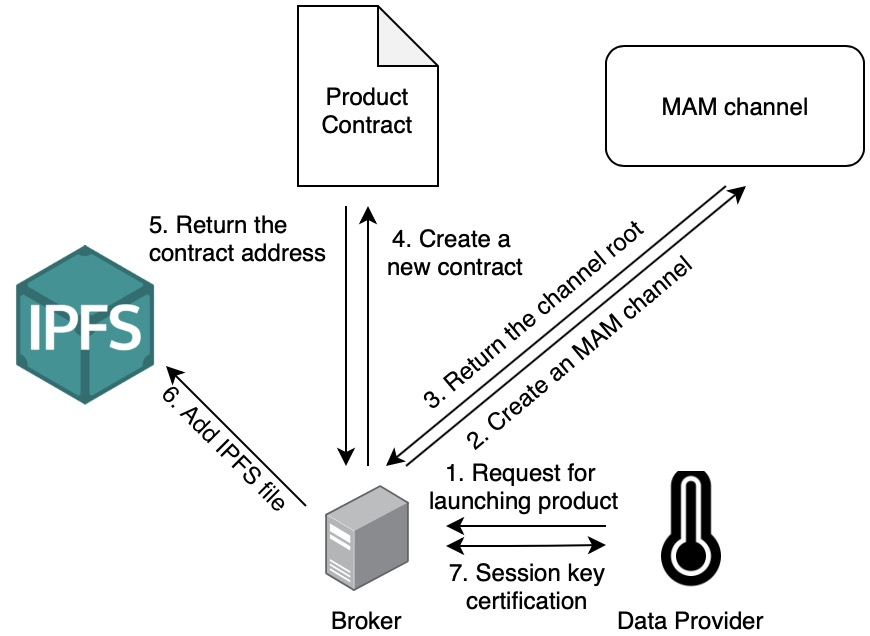
\includegraphics[width=3.3 in]{launching_product}
    \caption{The process of launching a product.}
    \label{fig:launching_product}
\end{figure}

\item \textbf{TangleID: }
The TangleID\cite{TangleID} is a self-sovereign identity system based on IOTA that does not require any third-party authority to verify an identity and its digital footprint. With TangleID, the digital footprint is converted into digital assets under the principle of Decentralized Identifiers (DIDs)\cite{DID} defined by W3C. Posting DID documents on MAM makes TangleID a GDPR-Complianced system\cite{GDPR}. Every participant in the data marketplace registers on TangleID, hence one can easily verify data providers' identity to ensure the data persistency from data sources.

Within the data darketplace, every entity generates a public/private key pair. Public MAM channel is created and its root address becomes part of the user ID, which at the same time serves as DID with the purpose to publish the public key of the entity. Private key along with the channels seed is locally stored in the local database of the entity. The public key of an entity can be used by others to encrypt sensitive data, that should only be accessible only by the entity. This is enabled via asynchronous encryption, where messages that are encrypted with a public key can only be decrypted with the matching private key.

The digital identities are also used to establish trust between the communication partners. This is done on two levels, proof that the communication partner owns the DID and the partner can, optionally, proof that it is a trusted participant. This authentication process happens during the first messages of interaction. In order for one partner to listen to another, it authenticates the messages. The DID ownership authentication is done by proving a digitally signed copy of the DID document.

The authentication of trust between the two parties is based on a Verifiable Credential, given out by a trusted issuer for the receiving party. If the receiving party does not trust the issuer, the credential is deemed worthless. If the party is recognized, the credential is verified and the messages will be labelled as trusted. In order the acquire this credential, the party needs to contact the issuer and ask for the credential. The issuer will need to know the DID of the party. If they decide to give out the credential, the issuer will sign the credential and send it encrypted over the blockchain to the requesting party's communication address. This is listed as a Service Endpoint (DID standard) in the DID Document of the requesting party.

\item \textbf{Ethereum Smart Contract: }
Smart contract is a protocol for formulating agreement on a blockchain that provides verification and execution of the contract. The code in the smart contract can interact with other contracts, make decisions, store data and transfer cryptocurrency. All conditions and states established in the contract are transparent and with enforcement. The appearance of smart contracts makes trading more flexible, and achieves more complex trading patterns in reality.

The Product Contract is used during the trading process, where Product Contract records all the details of data products, such as MAM channel's and endpoint's ID, blinded session key and data providers' DID Document address. Furthermore, data providers and consumers exchange session key through Product Contract without brokers' help. Though this design may cost more transaction fee than doing so off-chain, it is considered a better strategy to assure the profit of both providers and consumers. The further details of key exchangement will be illustrated in Section~\ref{section:trading}.

\item \textbf{Blind Signature}
There is an inherent risk in revealing session keys to brokers since contents may be copied by brokers, which would result in data providers' losses. Therefore, a blind signature is used to prevent session key copying for such circumstances. Blind signature\cite{blindSig} is a form of digital signature where the message is first "blinded" by a random "blinding factor", then passed to a signer to sign. Figure \ref{fig:blind_signature} illustrates the steps of blind signature. The resulting message, along with the blinding factor, can be later verified with the signer's public key. In our system design, brokers would perform blind signatures during the process of adding new products for data providers, in order to send the secret key of the MAM channel to the smart contract without knowing it.

\begin{figure}[h]
	\centering
	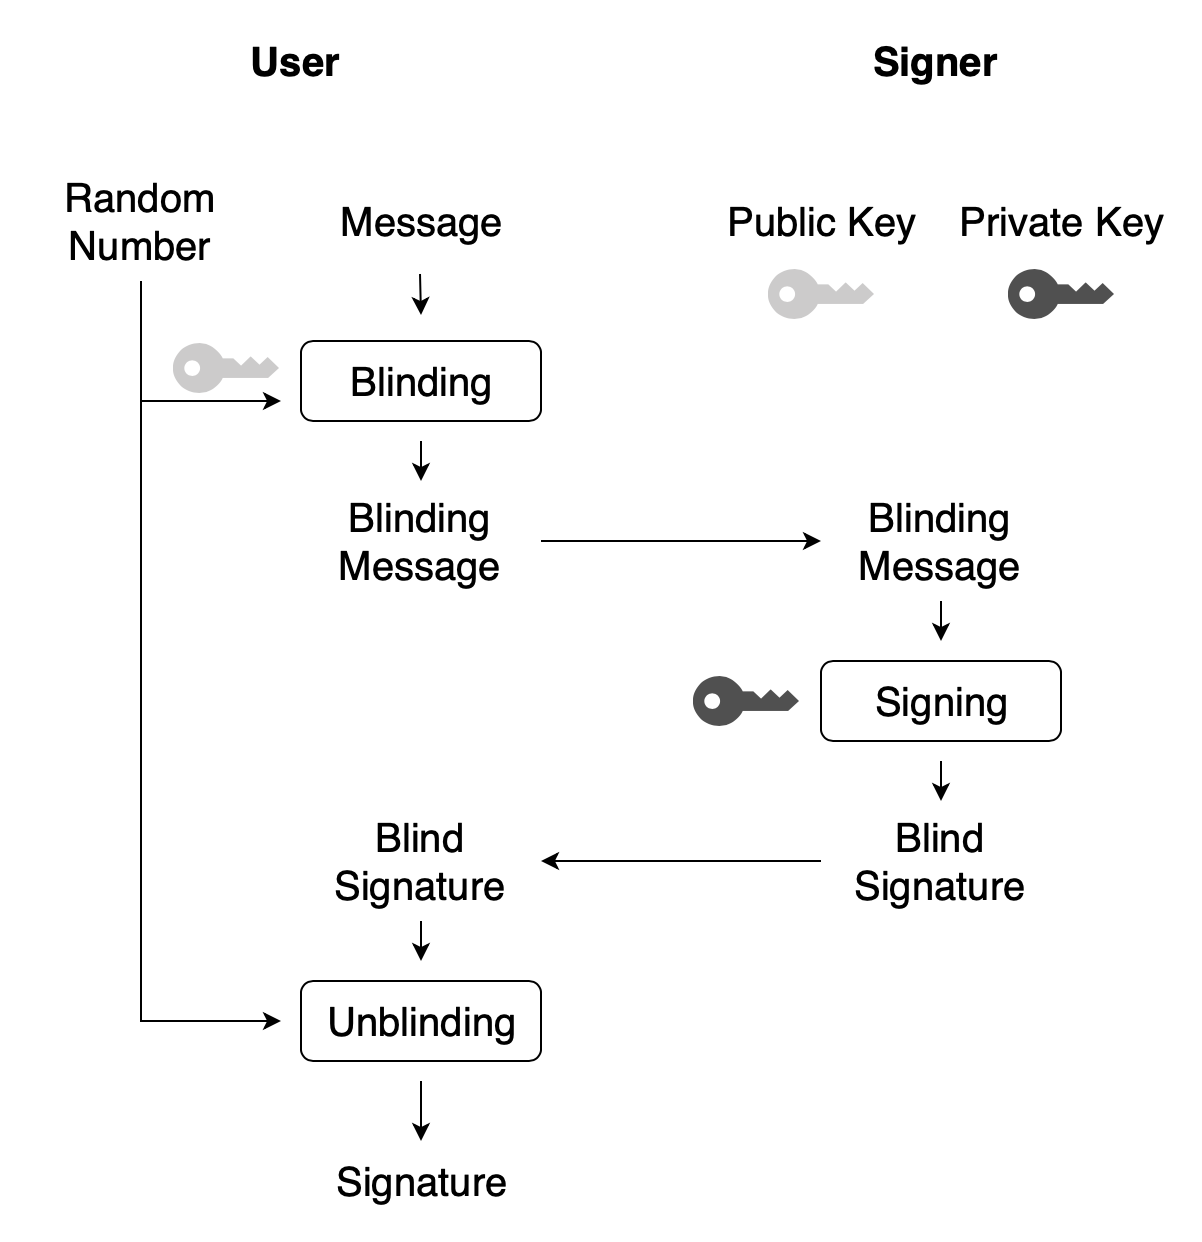
\includegraphics[width=3.3 in]{blind_signature}
	\caption{The scheme of blind signature.}
	\label{fig:blind_signature}
\end{figure}

RSA blind signature\cite{cryptoNote} is used in our research. The user chooses a random number $r$ and uses the signer's public key $e$ to generate a blinding factor $r^e$. To prevent the message $m$ from being known by the signer, the user sends blinding message $c$ to the signer instead of $m$.

\begin{equation}
C = r^e m
\end{equation}

The signer signs the blinding message with his private key $d$.

\begin{equation}
S = C^d
\end{equation}

$S$ is the signer's signature of $C$. In RSA system, $ed$ is equal to 1. To remove the blinding factor, the user computes the following calculation.

\begin{equation}
\frac{S}{r}= \frac{C^d}{r} = \frac{(r^e m)^d}{r} = \frac{r^{ed} m^d}{r} = m^d
\end{equation}
 
The user gets $m^d$ which is the signer's signature of the message $m$. At the same time, the signer does not know $m$ and the session key is protected. 

\item \textbf{IPFS}
Inter-Planetary File system(IPFS)\cite{IPFS} is a peer-to-peer network for storing and accessing files, websites, applications, and data in a distributed file system which is not maintained with certain nodes or entities but is with all IPFS users. In our proposed architecture, brokers are responsible to publish the metadata of products, including title, data provider information and data preview to the IPFS in order to provide users with search capabilities to meet the consumers' need.
\end{itemize}

\subsection{Trading Model}
In the following, we describe the data trading process in detail where we use game theory to ensure the sustainability of our trading model. To participate a data marketplace, data providers and consumers have to register first. Then data provider can launch its product on the marketplace. Once a product is launched, it is searchable and can be subsequently traded. The whole trading and refunding process is defined in smart contracts which are easily traceable and irreversible.

The consumer will pay for the data, only when the data sold by the data provider sufficiently accurate, for which we called such data "decent data."
Once the accuracy is lower than a certain threshold, which we call "unacceptable data," the consumers would then consider this data provider as a low quality data provider, and stop buying data from this data provider.

Refunds are a major issue in our research. However, we do not need to take refund as a factor in our game theory model, since in our decentralized data marketplace we use a smart contract to store the subscription fee which will be paid to buy the future data. The subscription fee will be paid as new data is transmitted to consumers. In other words, the data provider does not need to perform any procedures to transfer subscription fees from his/her own account to consumers' accounts. For the same reason, data providers have no responsibility on refunding processing fees charged by the smart contract.

\subsubsection{Participant Registration}
At the beginning, the registrar creates a registration contract, which maintains all participants' information, including their DID documents and public keys. Anyone can query participants' public keys. Those who would like to sell or purchase data may register to become a data provider or consumer. The registrar has the authority to agree with applications. After that, their identities are available in the registration contract and the launching and trading processes can begin.

\subsubsection{Launching and Searching Products}
To sell streaming data, a data provider needs to launch a new product on the data marketplace in advance as shown in Figure \ref{fig:launching_product}. The data provider determines a trusted broker and asks the broker to create a new MAM channel and product contract. Each product has a product contract to record the participants, subscription price brokerage fee, quantity of data and  trading process.

Brokers certify session keys as well. Only one session key can be signed in each product, so data providers cannot fake a session key to deceive consumers. Figure \ref{fig:key_certification} shows the certification process. When a data provider asks a broker to certify new session key $k$, the data provider uses the broker's public key, which is available in the Registration Contract after the broker's registration, as a blinding factor, and the session key is blinded. Then the data provider sends the blinded session key $Blind(k)$ to the broker. The broker signs the message and returns the signature $Sign(Blind(k))$ to data provider. The data provider removes the blinding factor and obtains the broker's signature of the session key, $Sign(k)$, which is verifiable by consumers.

\begin{figure}[H]
    \centering
    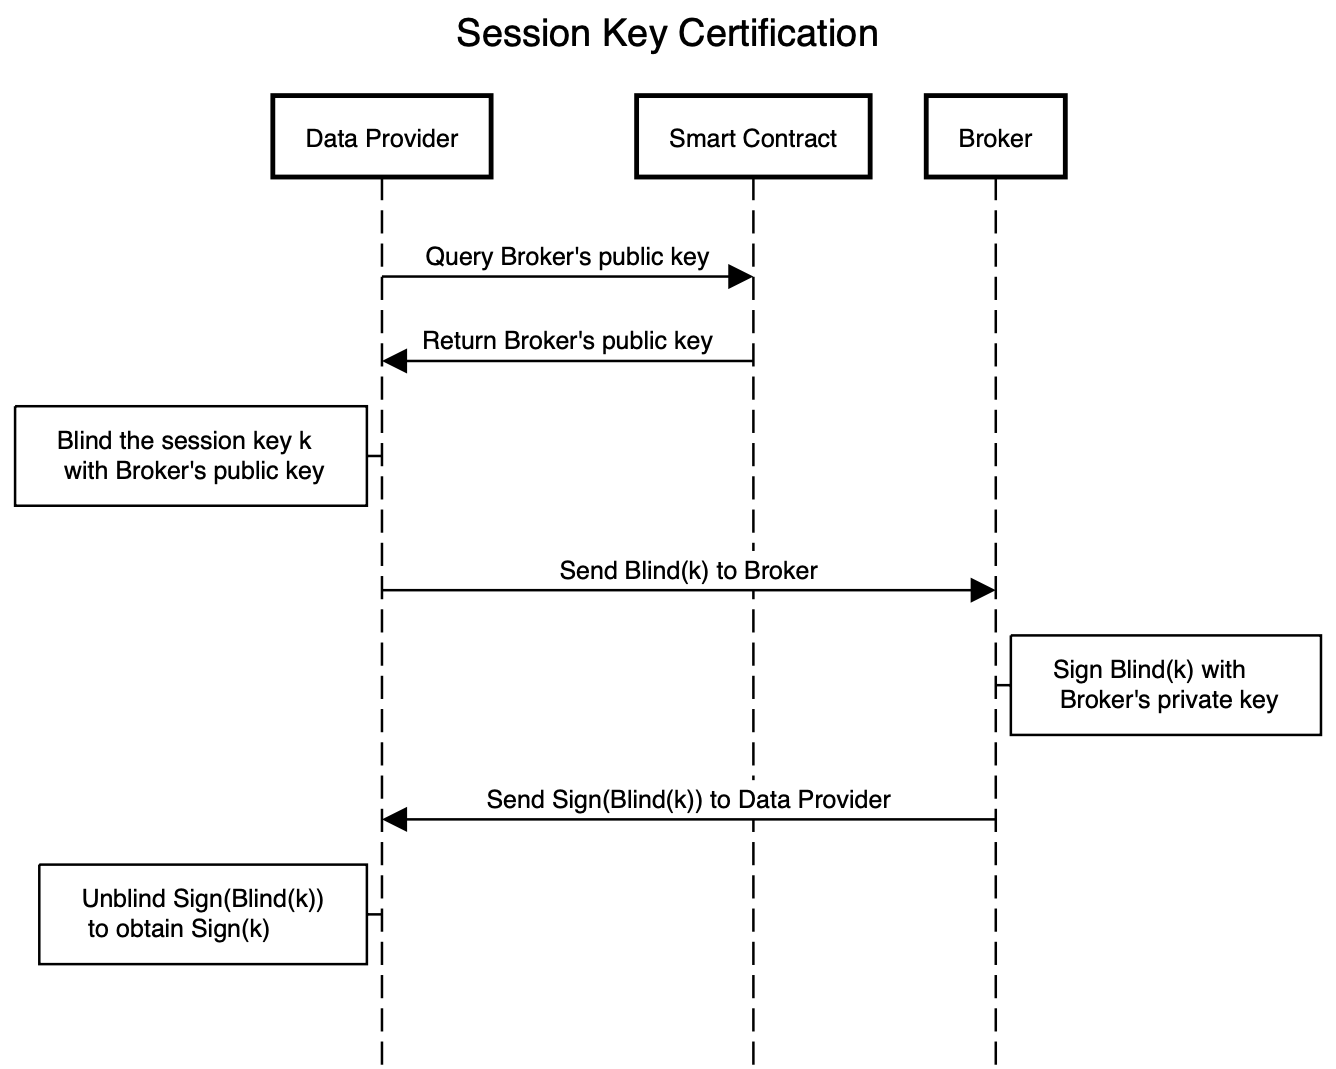
\includegraphics[width=4.4 in]{key_certification}
    \caption{Session key certification process with blind signature.}
    \label{fig:key_certification}
\end{figure}

The contract address and product description will be stored in a file which is uploaded to IPFS. Consumers can search the desired product by keywords or tags. In other words, the narrative description provides an entry to IoT world as end-users are able to label and search data they need based on the abstraction from IPFS files. Hence, the consumer then evaluates the product and initiates the trading with the data provider if the consumer is interested in subscribing to the data.

\subsubsection{Trading}
\label{section:trading}

The entire trading process is as shown in Figure \ref{fig:trading_product}. Once a consumer wants to subscribe certain streaming data that is generated, he/she has to pay subscription fee to the Product Contract and will be automatically added on the list by the smart contract.

\begin{figure}[H]
    \centering
    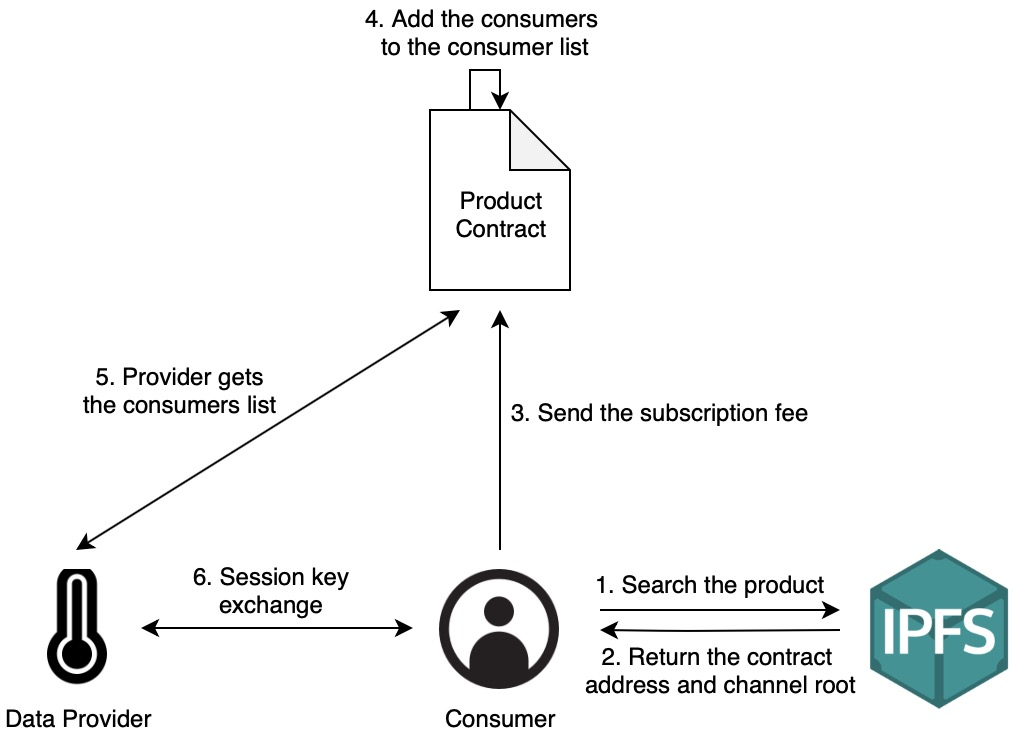
\includegraphics[width=3.3 in]{trading_product}
    \caption{The process for the product trading.}
    \label{fig:trading_product}
\end{figure}

Next, session key $k$ should be exchanged between the data provider and consumers. To exchange data, Azaria et al\cite{Medrec} seek an off-chain solution which is based on an end-to-end communication to ensure the efficiency and low costs. However, it is hard to avoid that the data source is unavailable or the sender sends incorrect data intentionally. Instead of using off-chain solution, we use smart contract to transfer the session key\cite{3tierDataMarket} that not only ensures the consistency of the session key, the availability of the source and the traceability of the record, but also prevents malicious participants to cheat others.

\lstdefinestyle{solidity}{
	captionpos=b,
	tabsize=4,
	basicstyle=\scriptsize
}
\lstset{style=solidity}

\begin{lstlisting}[caption={update encrypt key}, label={lst:key_exchange}, frame=single]
    function addEncryptKey(
        address _consumer,
        string memory _encryptKey
    ) public {
        require(
            msg.sender == provider,
            "Only provider can add blindedKey."
        );
        require(
            consumer2Purchase[_consumer].isKeyAdded == false,
            "One encryptKey has been added."
        );
        consumer2Purchase[_consumer].encryptKey = _encryptKey;
        consumer2Purchase[_consumer].isKeyAdded = true;
        emit newEncryptKey(_consumer, _encryptKey);
    }
\end{lstlisting}

The trading process is shown in Figure \ref{fig:key_exchange}. The data provider can obtain public keys of each consumer from the registration contract. For each consumer, the data provider encrypts the session key and broker's signature with the consumer's public key and sends the ciphertext $Encrypt(k + Sign(k))$ to the product contract by calling $addEncryptKey()$ (Listing \ref{lst:key_exchange}). Consumers listen to the $newEncryptKey$ event which is triggered when the ciphertext is updated, and decrypt the ciphertext to obtain the session key $k$ and signature $Sign(k)$.

\begin{figure}[H]
    \centering
    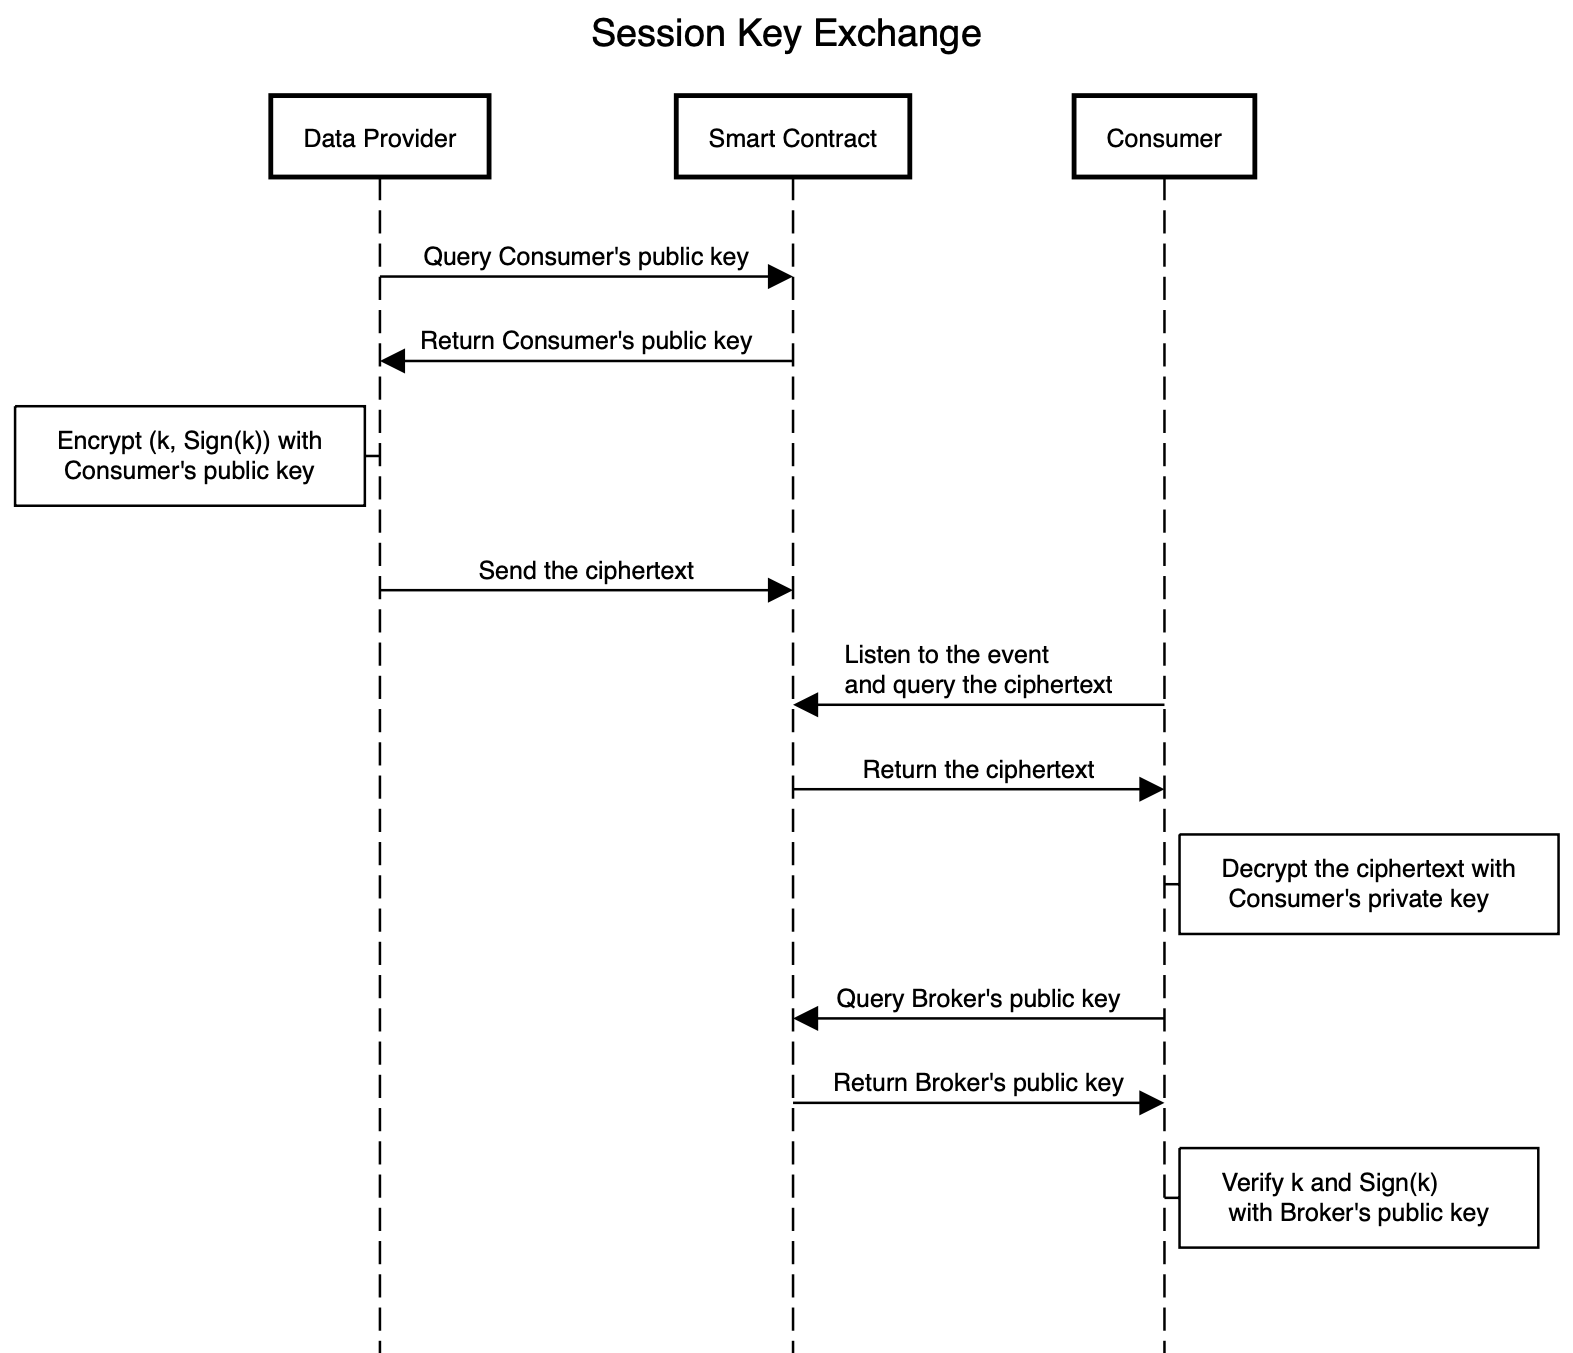
\includegraphics[width=5.5 in]{key_exchange}
    \caption{Session key exchange process between the data provider and consumer.}
    \label{fig:key_exchange}
\end{figure}

Consumers can obtain the broker's public key on the registration contract as well, so they can verify that the signature is valid and the session key is the only one that is certified by the broker. Afterward, encrypted data is published to the MAM channel, and consumers can obtain and decrypt it with the session key.

\subsubsection{Refunding}

It is probable that the streaming data sources are delayed or even interrupted after the consumers pay the subscription fee. To protect consumer rights, the subscription fee are not transferred to the data provider until data is generated and published to the MAM channel. If the expected data is not available, consumers can request refunds. We assume that a very small percentage of consumers in the product contract are irrational and/or malicious. When a consumer consents to refund, he can vote at any time. After the ratio of consent votes of refunding is higher than the $threshold$, the subscription fee is proportionally transferred to the data provider, broker and every consumer. Figure \ref{fig:refund} shows the refund process.

\begin{figure}[h]
	\centering
	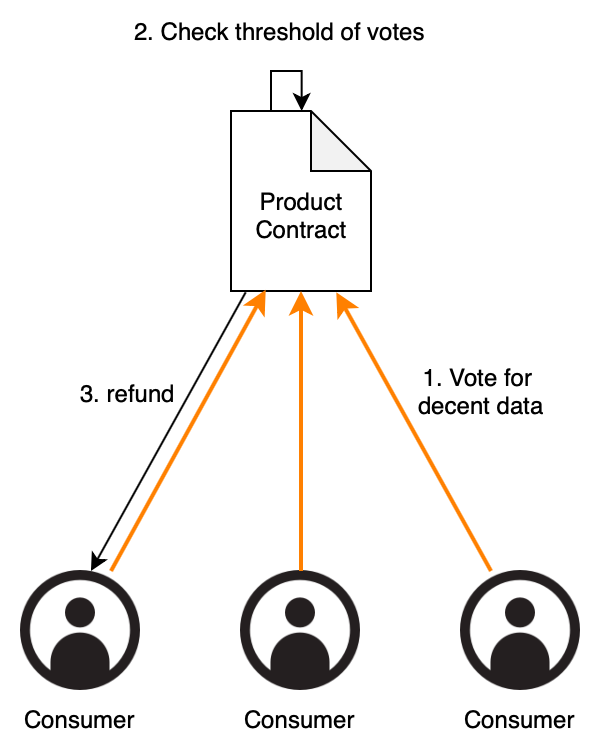
\includegraphics[width=2 in]{refund}
	\caption{The process of refund.}
	\label{fig:refund}
\end{figure}

The subscription fee can be prorated as below:

\begin{equation}
    F_{DataProvider}(i) = N price \frac{i-1}{M} (1-F_{b}) -F_{t}
\end{equation}

\begin{equation}
    F_{Broker}(i) = N price \frac{i-1}{M} F_{b} -F_{t}
\end{equation}

\begin{equation}
    F_{Consumer}(i) = price \frac{M-i+1}{M} -F_{t}
\end{equation}

where $i$ is the number of data when refunding condition is met, $price$  is the subscription price, $M$ is the number of expected data samples, $F_{b}$ (\%) is the brokerage fee which is expressed as a percentage, $F_{t}$ is the transaction fee of the smart contract, $N$ is the number of consumers in this contract.

To refund or withdraw subscription fees from the smart contract, the data provider, broker, and consumer send a transaction to execute the smart contract and are responsible for the transaction fee. We assume that only a half of the expected records are published to the MAM channel. When $F_{b}$ is 5\%, the data provider and broker can withdraw half of the total subscription fee from the smart contract and 5\% of the subscription fee belongs to the broker while the remaining belongs to the data provider. For consumers, they can receive half of the subscription fee refunded which should be deducted from the transaction fee.

Considering the situation that one of the consumers requests a refund in the future, when the consumer is disappointed with the data quality, he/she may request a refund.

\subsubsection{Game Theory Adoption}
Game Theory is a methodology to discuss strategic interaciton among game players. If we can ensure Nash Equilibrium of decentralized data marketplace exists at a certain acceptable range, then we can promise the sustainability of decentralized data marketplace. Fan Liang et al\cite{SurveyBigDataPricing} listed several different types of game theory models which are applied to data pricing. We employed repeated games to build our game theory model. Repeated games consists of several repetitions of the same base game which meets the scenario of data subscription.

Figure \ref{fig:decision_tree} shows the decision tree to depict the repeated game we used. Each level in this decision tree represents each round of data transmission from data provider to consumers, and the consumers would pay subscription fee, $p_s$, for each person. The sum of all the subscription fee paid to the data provider is denoted as $P_s$.

\begin{figure}[H] \centering 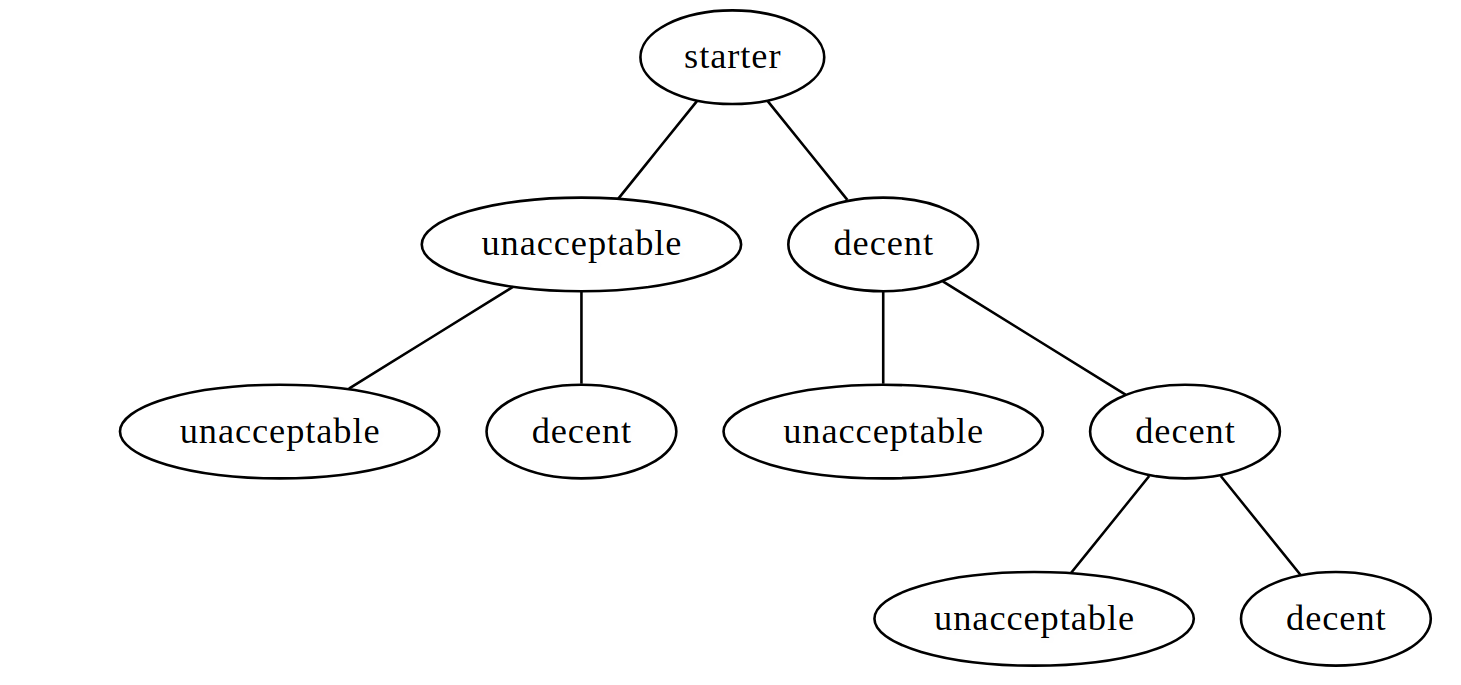
\includegraphics[width=3.3 in]{decision_tree} \caption{Decision Tree}
    \label{fig:decision_tree} \end{figure}
For every $n$ round, the data provider would pay the maintenance fee, $C_{maintain}$, to as the incentives of maintaining or enhancing the sensors that the data provider owns. We call this a maintenance period. Moreover, the cost of maintenance will decrease as time passes, so we introduce a discounted factor $\beta$ to depict this phenomena.

Following assumptions are made:
\begin{enumerate}
    \item  We assume consumers are rational. \label{rational_man}
    \item  Each data provider is the sole provider of the product they produced. \label{monopoly}
    \item  Subscription fees only depends on data quality. \label{fee_vs_quality}
    \item  At least 51\% of consumers are in the same group which has complete information exchange.\label{51_in_group}
    \item  One of the consumers who has complete information exchange with other 51\% buyers has the ability to examine data quality. \label{1_in_51}
\end{enumerate}

According to \textbf{assumption(\ref{rational_man})}, we learn that few consumers would take malicious actions in this system, since all the consumers are rational. For most of the rational consumer, they can't obviously benefit from collapsing of Data Marketplace.

\textbf{Assumption(\ref{monopoly})} implies there is no other data providers providing the same product in the data marketplace. In this way, we can consider each provider's behavior independently. That means this decision tree represents the behavior of only one data provider. Price war between data providers is not under consideration here.

From \textbf{assumption(\ref{51_in_group})}, we derive that if one of any consumer in that group of complete information exchange consumers launches voting for stopping buying data (in other words, the consumer announces the data quality is not acceptable), they would succeed in rejecting the processing subscription.

\textbf{Assumption(\ref{1_in_51})} implies if unacceptably low quality data are delivered to consumers, the examiner will be aware of the unacceptable data quality and spread this information out.


Based on the description above, the discounted sum of payoff for our repeated game is
\begin{equation} \label{payoff}
    \sum_{i=0}^{m - 1}{\beta^{in}\cdot [(\sum_{j=0}^{n - 1} \beta^j \cdot P_s) - C_{maintain}]}
\end{equation}

Al-Fagih et al. presented\cite{DataPrice} the sum of the subscription fee, $P_s$, is sigmoid function of data quality, $P_r$, and based on rule of thumb, $C_{maintain}$ is approximately an exponential function of $P_r$. We can substitute $P_s$ and $C_{maintain}$ with $P_r$ into Eq. (\ref{payoff}). With the resulting equation, we can find out the Nash Equilibrium of repeated game.

\subsubsection{Numerical Example}
To evaluate the behavior of the game theory model we just presented, first, we would express the function of $P_s$ and $C_{maintain}$ as functions of $P_r$ respectively. Therefore, the sum of subscription fee of all subscriber can be expressed as

\begin{equation} \label{sub_fee}
    P_s = R \frac{e^{a (P_r - b)}}{1 + e^{a (P_r - b)}}
\end{equation}

where $a$ and $b$ are tuning factors, and $R$ is the maximum possible data value.

And we would express the cost of maintenance as

\begin{equation} \label{C_mtn}
    C_{maintain} = ce^{P_r - d}
\end{equation}
Where $c$ and $d$ are tuning factors.

Substitute Eq. (\ref{sub_fee}) and Eq. (\ref{C_mtn}) into Eq. (\ref{payoff}). We can derive
\begin{equation} \label{payoff_Pr}
    \sum_{i=0}^{m - 1}{\beta^{in}\cdot [(\sum_{j=0}^{n - 1} \beta^j \cdot R \frac{e^{a (P_r - b)}}{1 + e^{a (P_r - b)}}) - ce^{P_r - d}]}
\end{equation}

\begin{figure}[H] \centering 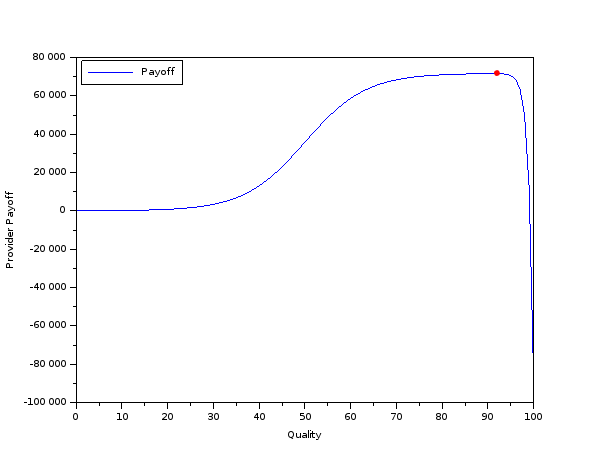
\includegraphics[width=3.3 in]{payoff_pic} \caption{Payoff Function}
    \label{fig:payoff_pic} \end{figure}

The red dot in Figure \ref{fig:payoff_pic} indicates the data quality that data provider would sustain, since the data provider can achieve maximum payoff at that point. Namely, the red dot is the Nash Equilibrium of this game theory model.

Figure \ref{fig:payoff_pic} illustrates the market mechanism of the subscription trading policy we used under the decentralized data marketplace. First, data providers have weak motivation to operate their sensor in low accuracy, since the incentive of low quality data is much less than moderate quality data. Second, the great deficit at high accuracy is mostly derived by the rapid increasing of maintenance cost. Thus, if the maintenance fee to achieve decent data quality is under a fair price range, then data provider will automatically provide data with high enough data quality under our assumptions.


\section{Evaluations}
It is worth making a claim that all participants in data marketplace do not need to hold an IOTA full node which maintains the transaction history and exchanges information of the Tangle. Each role is only required to run client libraries and communicate with IOTA full nodes to interact with the Tangle. Therefore, in the following evaluations, all devices run with client library only.

\subsection{MAM Performance Evaluation}
MAM is a secure and validatable data storage of the proposed architecture. And publishing data to MAM is the primary key to resolve all the difficulties discussed in previous sections. The interactions between data providers and MAM can be frequent. Data providers can either upload data in a short time interval or maintain multiple MAM channels or endpoints at the same time, hence the operation of MAM is one of the bottleneck in data marketplace.

In this section, time measurement is evaluated in two MAM operations: channel/endpoint creation and data attachment to endpoints. To perform the evaluation assessment, a personal computer and a Raspberry Pi 3 have been used to run MAM. 

\subsubsection{Channel / Endpoint Creation}
The length of a channel or endpoint is $2^{height}$ where \textit{height} is the height of Merkle Hash Tree in Merkle signature scheme (MSS). A channel with height $n$ can create $2^n$ endpoints, and an endpoint with height $m$ can attach $2^m$ messages, therefore the capacity of a channel is $2^{nm}$ messages in total. The greater the \textit{height} of MSS, the longer the channel/endpoint, however the higher the computational power required. In this task, both channel and endpoint creation are tested and the \textit{height} is set from 1 to 7 which is quite enough for data providers to upload data. The results are shown in Table \ref{tab:channel_create} and Table \ref{tab:endpoint_create}. The time duration for each \textit{height} is the average time of running 100 rounds.

\begin{table}[H]
	\caption{Time measurement of channel creation}
	\centering
	\label{tab:channel_create}
	\begin{tabular}{ccc}
	\toprule
		\textbf{height of MSS} & \textbf{PC (sec)} & \textbf{Raspberry Pi 3 (sec)} \\ 
		\midrule
		1 & 0.26183 & 2.908702 \\ 
		2 & 0.524076 & 5.805524 \\ 
		3 & 1.045942 & 11.555660 \\ 
		4 & 2.092989 & 23.178036 \\ 
		5 & 4.19515 & 46.164079\\ 
		6 & 8.361586 & 92.320173\\ 
		7 & 16.651607 & 185.292243\\
		\bottomrule
	\end{tabular}
\end{table}

\begin{table}[H]
	\caption{Time measurement of endpoint creation}
	\centering
	\label{tab:endpoint_create}
	\begin{tabular}{ccc}
	\toprule
		\textbf{height of MSS} & \textbf{PC (sec)} & \textbf{Raspberry Pi 3 (sec)} \\ 
		\midrule
		1 & 0.256425 & 2.887064 \\ 
		2 & 0.505679 & 5.767912 \\ 
		3 & 0.999524 & 11.550455 \\ 
		4 & 1.994017 & 23.260508 \\ 
		5 & 3.965007 & 46.748366 \\ 
		6 & 7.918925 & 93.182975 \\ 
		7 & 16.561419 & 186.064562 \\
		\bottomrule
	\end{tabular}
\end{table}

The results in Table \ref{tab:channel_create} and Table \ref{tab:endpoint_create} are plotted in Figure \ref{fig:mam_create}. Since the creation of channel and endpoint are MSS calculation, the curves of the same hardware are merely identical. On the other hand, the performance of Raspberry Pi 3 grows rapidly when \textit{height} is larger.
  
\begin{figure}[H]
    \centering
    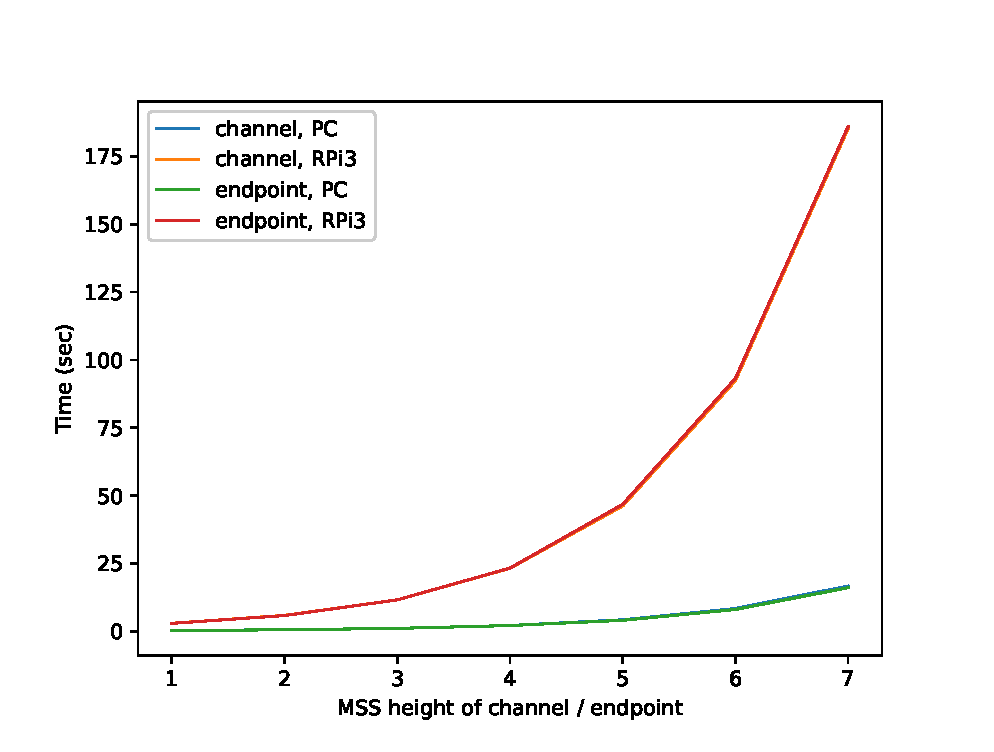
\includegraphics[width=3.3 in]{mam_create}
    \caption{Time cost of MAM creation.}
    \label{fig:mam_create}
\end{figure}

\subsubsection{Messages Publishment}
Publishing a message to MAM is attaching a zero-value transaction to the Tangle which requires two processes:
\begin{itemize}[leftmargin=*,labelsep=5.8mm]
	\item	Tips selection: In IOTA protocol, a new-coming transaction needs to pick up 2 existed transactions called tips to reference and verify. The tips are provided by IOTA full nodes.
	\item	Proof-of-Work (PoW): Perform a series of mathametic calculation for the transaction in order to be validated.
\end{itemize}

Tips selection requires a stable network connection to wait the response from IOTA full nodes, and PoW requires enough computation resources to perform. Figure \ref{fig:mam_send} shows PDF of publishing one message to MAM endpoint for 100 times. The average time for PC to send a message is 48.1069 seconds, and Raspberry Pi 3 takes 743.8586 seconds.

\begin{figure}[H]
    \centering
    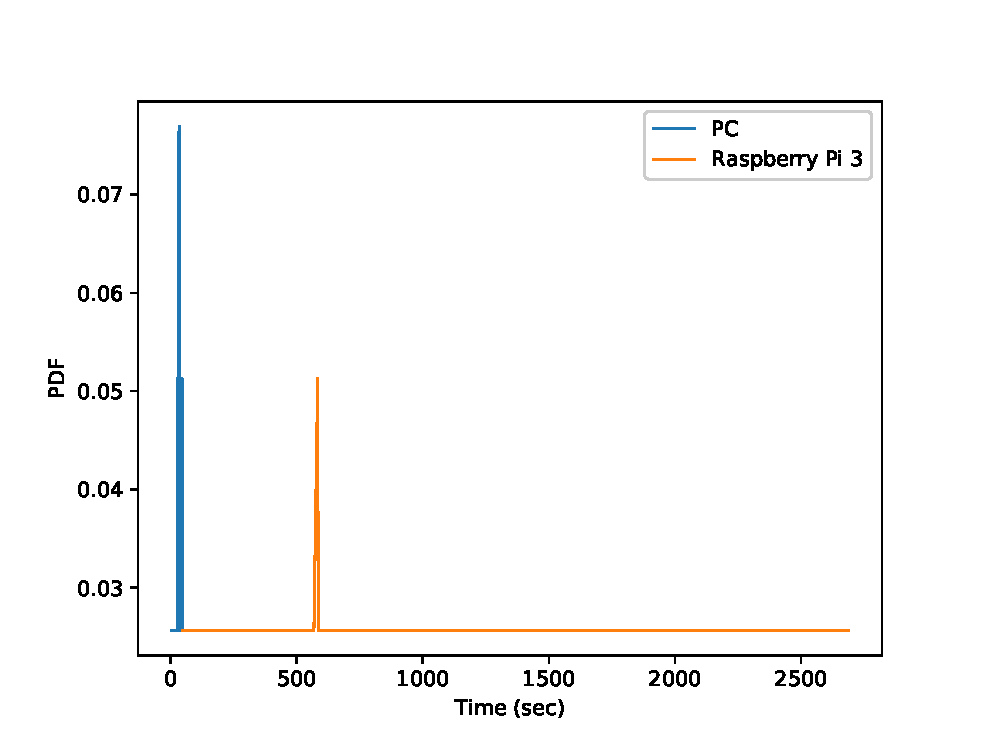
\includegraphics[width=3.3 in]{mam_send}
    \caption{Time cost of sending a message through MAM.}
    \label{fig:mam_send}
\end{figure}

MAM operations take a lot of time for both devices, but Raspberry Pi 3 spends even more time than PC. The simulation results above indicate that MAM is difficult for low-level sensor devices to run, which these devices are the majority hardware as data providers in the data marketplace. Furthermore, sensors with the low computing power and weak internet connection are not able to have enough resources to handle data collection, data transmission on MAM and trading process with consumers simultaneously. Therefore, transferring MAM operations to brokers, which can be PCs or even more powerful machines, while ensuring the profit of providers can effectively solve performance problems and lower the threshold for participation in the data marketplace. However, even on PC, MAM operations still cost a considerable time, improving the performance is an essential issue that needs to be done for the next step.  



\subsection{Smart Contract}

In this experiment, we investigate the cost of executing smart contracts. We implement the smart contract and measure gas(transaction fee of the Ethereum blockchain) usage. There are transaction cost and execution cost associated for an Ethereum transaction. We focus on execution cost which is included in transaction cost.

\begin{lstlisting}[caption={generate contract}, label={lst:constructor}, frame=single]
	constructor(
		address _provider,
		uint _price,
		uint _brokerage,
		uint _threshold,
		string memory _channelRoot,
		string memory _endPoint,
		uint256 _totalNumber
	) public {
		broker = msg.sender;
		provider = _provider;
		isBrokerWithdraw = false;
		isProviderWithdraw = false;
		price = _price;
		totalAmount = 0;
		brokerage = _brokerage;
		threshold = _threshold;
		channelRoot = _channelRoot;
		endPoint = _endPoint;
		totalNumber = _totalNumber;
		uploadedNumber = 0;
		state = State.Launched;
	}
\end{lstlisting}

To create a Product Contract (Listing \ref{lst:constructor}), metadata such as the address of the data provider, subscription fee, brokerage fee, threshold of consent votes of refunding, the channel root and endpoint of MAM channel, and expected number of streaming data should be defined and initialized when the contract is deployed by the broker. A Product Contract also records the process of session key certification and exchange, and prevents transactions of invalid behaviors, such as certifying multiple session keys by the data provider to cheat consumers, from changing the contract state.

\begin{lstlisting}[caption={update blinded key and update signature}, label={lst:key_certification}, frame=single]
	function addBlindedKey(
		string memory _blindedKey
	) public {
		require(
			msg.sender == provider,
			"Only provider can add blindedKey."
		);
		require(
			state == State.Launched,
			"One key has been certified."
		);
		blindedKey = _blindedKey;
		emit newBlindedKey(blindedKey);
	}
	
	function addSignedBlindedKey(
		string memory _signedBlindedKey
	) public {
		require(
			msg.sender == broker,
			"Only broker can add signedBlindedKey."
		);
		require(
			state == State.Launched,
			"One key has been certified."
		);
		signedBlindedKey = _signedBlindedKey;
		state = State.KeyCertified;
		emit newSignedBlindedKey(signedBlindedKey);
	}
\end{lstlisting}

Before a data provider asks a broker to certify a session key, he blinds the session key first. The blinded session key is published to the smart contract by calling $addBlindedKey()$(Listing \ref{lst:key_certification}). Also the broker should use $addSignedBlindedKey()$(Listing \ref{lst:key_certification}) to publish the signature. As a result, the key certification process is recorded on the smart contract which is traceable afterward. By the way, it is hard for an attacker to compute the session key with blinding messages and signatures on smart contracts.

\begin{table}[H]
	\caption{Gas consumption for each function of Product Contract}
	\centering
	\label{tab:gas}
	\begin{tabular}{cccc}
		\toprule
		\textbf{function} & \textbf{sender} & \textbf{transaction cost (gas)} & \textbf{execution cost (gas)} \\
		\midrule
		generate contract & Broker & 2954334 & 2251002 \\
		subscribe product & Consumer & 65758 & 44486 \\
		update blinded key & Provider & 180801 & 147369 \\
		update signature & Broker & 201110 & 167678 \\
		update encrypt key & Provider & 201624 & 166784 \\
		update number & Broker & 54289 & 32825 \\
		ask refund & Consumer & 43817 & 22545 \\
		withdraw & Broker/Provider/Consumer & 35991 & 14719 \\
		\bottomrule
	\end{tabular}
\end{table}

Table \ref{tab:gas} shows the gas usage for each function. Creating a smart contract (Listing \ref{lst:constructor}) costs the most gas, and functions (Listing \ref{lst:key_exchange} and Listing \ref{lst:key_certification}) that are related to key certification and key exchange need a lot of gas as well. Storage on blockchain costs a lot. It is expensive to use memory in Solidity. For instance, an SSTORE operation may cost 20000 gas when the value is set to non-zero from zero according to Ethereum Yellow Paper\cite{Ethereum}. Smart contract initialization, storing ciphertexts and signatures during key certification and key exchange needs a lot of operations and storages which causes high gas consumption. To certify session keys, blind signature is used and the whole process is recorded in the smart contract. However, storage on blockchain is expensive and blind signature is an interactive protocol which requires multi-steps of communications between broker and data provider. In our future work, we are going to explore the usage of the non-interactive zero knowledge protocol such as zk-SNARKS(zero-knowledge succinct non-interactive argument of knowledge)\cite{Snark} which can generate proofs off-chain and simplify the verification process that could not only reduce network and storage cost but also improve the privacy and security of session keys. On the other hand, we can observe that the broker is responsible for the most part of transaction fees while consumers only need to send one transaction to subscribe the product if they do not have to refund.

%%%%%%%%%%%%%%%%%%%%%%%%%%%%%%%%%%%%%%%%%%
%Bulleted lists look like this:
%\begin{itemize}[leftmargin=*,labelsep=5.8mm]
%Numbered lists can be added as follows:
%\begin{enumerate}[leftmargin=*,labelsep=4.9mm]


%%%%%%%%%%%%%%%%%%%%%%%%%%%%%%%%%%%%%%%%%%
\section{Conclusions}

By combining the established standards and openly-developed specifications, this paper proposed an autonomous data marketplace design to serve as a vendor and industry-neutral platform, automating the trading of digital assets and services. It was built with blockchain network, immutable audit trails, and contracts with an integrated decentralized identity system, to ensure the authenticity of all participants and enable secure communication and flexible trading mechanisms.

%Data Auction
The data auction process is a data trading mechanism and an economically-driven scheme that establishes corresponding prices of data products through bidding process between consumers and providers. While there has been many auction models\cite{BigPicDataMarket} in several areas, there has been minimal research on third-party auction platforms. Our proposed decentralized data marketplace protects the privacy of participants which reveals the minimum information for validation and reduces the suspicion of trust to centralized parties or auctioneers. However, the auction process between multiple participants and analysis of potential threats are still critical issues that need to be resolved. For the game theory model presented in this work, we assume each data provider's behavior is independent. However, normally there would be multiple data providers providing similar products (substitutions). Only one provider is taken into considerations at present.


%%%%%%%%%%%%%%%%%%%%%%%%%%%%%%%%%%%%%%%%%%
\reftitle{References}

% Please provide either the correct journal abbreviation (e.g. according to the “List of Title Word Abbreviations” http://www.issn.org/services/online-services/access-to-the-ltwa/) or the full name of the journal.
% Citations and References in Supplementary files are permitted provided that they also appear in the reference list here. 

%=====================================
% References, variant A: external bibliography
%=====================================
\externalbibliography{yes}
\bibliography{references}

%=====================================
% References, variant B: internal bibliography
%=====================================
%\begin{thebibliography}{999}
%\bibliography{references}
% Reference 1
%\bibitem[Author1(year)]{ref-journal}
%Author1, T. The title of the cited article. {\em Journal Abbreviation} {\bf 2008}, {\em 10}, 142--149.
% Reference 2
%\bibitem[Author2(year)]{ref-book}
%Author2, L. The title of the cited contribution. In {\em The Book Title}; Editor1, F., Editor2, A., Eds.; %Publishing House: City, Country, 2007; pp. 32--58.
%\end{thebibliography}

% The following MDPI journals use author-date citation: Arts, Econometrics, Economies, Genealogy, Humanities, IJFS, JRFM, Laws, Religions, Risks, Social Sciences. For those journals, please follow the formatting guidelines on http://www.mdpi.com/authors/references
% To cite two works by the same author: \citeauthor{ref-journal-1a} (\citeyear{ref-journal-1a}, \citeyear{ref-journal-1b}). This produces: Whittaker (1967, 1975)
% To cite two works by the same author with specific pages: \citeauthor{ref-journal-3a} (\citeyear{ref-journal-3a}, p. 328; \citeyear{ref-journal-3b}, p.475). This produces: Wong (1999, p. 328; 2000, p. 475)


%%%%%%%%%%%%%%%%%%%%%%%%%%%%%%%%%%%%%%%%%%
%% optional
%\sampleavailability{Samples of the compounds ...... are available from the authors.}

%% for journal Sci
%\reviewreports{\\
%Reviewer 1 comments and authors’ response\\
%Reviewer 2 comments and authors’ response\\
%Reviewer 3 comments and authors’ response
%}

%%%%%%%%%%%%%%%%%%%%%%%%%%%%%%%%%%%%%%%%%%
\end{document}

